%%%%%%%%%%%%%%%%%%%%%%%%%%%%%%%%%%%%%%%%%
% Short Sectioned Assignment LaTeX Template Version 1.0 (5/5/12)
% This template has been downloaded from: http://www.LaTeXTemplates.com
% Original author:  Frits Wenneker (http://www.howtotex.com)
% License: CC BY-NC-SA 3.0 (http://creativecommons.org/licenses/by-nc-sa/3.0/)
%%%%%%%%%%%%%%%%%%%%%%%%%%%%%%%%%%%%%%%%%

% \documentclass[paper=a4, fontsize=11pt]{scrartcl} % A4 paper and 11pt font size
\documentclass[12pt, a4paper]{book}
\usepackage[T1]{fontenc} % Use 8-bit encoding that has 256 glyphs
\usepackage[utf8]{inputenc}
\usepackage{fourier} % Use the Adobe Utopia font for the document - comment this line to return to the LaTeX default
\usepackage{listings} % para insertar código con formato similar al editor
\usepackage[spanish, es-tabla]{babel} % Selecciona el español para palabras introducidas automáticamente, p.ej. "septiembre" en la fecha y especifica que se use la palabra Tabla en vez de Cuadro
\usepackage{url} % ,href} %para incluir URLs e hipervínculos dentro del texto (aunque hay que instalar href)
\usepackage{graphics,graphicx, float} %para incluir imágenes y colocarlas
\usepackage[gen]{eurosym} %para incluir el símbolo del euro
\usepackage{cite} %para incluir citas del archivo <nombre>.bib
\usepackage{enumerate}
\usepackage{hyperref}
\usepackage{graphicx}
\usepackage{tabularx}
\usepackage{booktabs}

\usepackage[table,xcdraw]{xcolor}
\hypersetup{
	colorlinks=true,	% false: boxed links; true: colored links
	linkcolor=black,	% color of internal links
	urlcolor=cyan		% color of external links
}
\renewcommand{\familydefault}{\sfdefault}
\usepackage{fancyhdr} % Custom headers and footers
\pagestyle{fancyplain} % Makes all pages in the document conform to the custom headers and footers
\fancyhead[L]{} % Empty left header
\fancyhead[C]{} % Empty center header
\fancyhead[R]{Pablo Jiménez Jiménez} % My name
\fancyfoot[L]{} % Empty left footer
\fancyfoot[C]{} % Empty center footer
\fancyfoot[R]{\thepage} % Page numbering for right footer
%\renewcommand{\headrulewidth}{0pt} % Remove header underlines
\renewcommand{\footrulewidth}{0pt} % Remove footer underlines
\setlength{\headheight}{13.6pt} % Customize the height of the header

\usepackage{titlesec, blindtext, color}
\definecolor{gray75}{gray}{0.75}
\newcommand{\hsp}{\hspace{20pt}}
\titleformat{\chapter}[hang]{\Huge\bfseries}{\thechapter\hsp\textcolor{gray75}{|}\hsp}{0pt}{\Huge\bfseries}
\setcounter{secnumdepth}{4}
\usepackage[Lenny]{fncychap}
\linespread{1.2}

\usepackage{glossaries}

\makeglossaries

\newglossaryentry{CIE-10}
{
    name=CIE-10,
    description={Es el acrónimo de la Clasificación internacional de enfermedades, 10.ª edición correspondiente.}
}

\begin{document}

	% Plantilla portada UGR
	\begin{titlepage}
\newlength{\centeroffset}
\setlength{\centeroffset}{-0.5\oddsidemargin}
\addtolength{\centeroffset}{0.5\evensidemargin}
\thispagestyle{empty}

\noindent\hspace*{\centeroffset}\begin{minipage}{\textwidth}

\centering

\includegraphics[width=0.9\textwidth]{doc/logos/logo_ugr.jpg}\\[1.4cm]

\textsc{ \Large TRABAJO FIN DE GRADO\\[0.2cm]}
\textsc{ GRADO EN INGENIERÍA INFORMÁTICA}\\[1cm]

\vspace{2cm}

{\Huge\bfseries Computación y optimización en la nube \\}
\noindent\rule[-1ex]{\textwidth}{3pt}\\[3.5ex]
{\large\bfseries Implementación de una aplicación de datos abiertos en la nube }
\end{minipage}


\noindent\hspace*{\centeroffset}
\begin{minipage}{\textwidth}
\centering

\textbf{Autor}\\ {Pablo Jiménez Jiménez}\\[2.5ex]
\textbf{Director}\\ {Juan Julián Merelo Guervós}\\[2cm]

\includegraphics[width=0.3\textwidth]{doc/logos/etsiit_logo.png}\\[0.1cm]
\textsc{Escuela Técnica Superior de Ingenierías Informática y de Telecomunicación}\\
\textsc{---}\\
Granada, 8 de julio de 2022
\end{minipage}
\end{titlepage}


	% Plantilla prefacio UGR
	\thispagestyle{empty}

\begin{center}
{\large\bfseries Computación y optimización en la nube \\ Implementación de una aplicación de datos abiertos en la nube }\\
\end{center}
\begin{center}
Pablo Jiménez Jiménez \\
\end{center}

%\vspace{0.7cm}

\vspace{0.5cm}
\noindent{\textbf{Palabras clave}: \textit{software libre, open source, API, OpenAPI, GraphQL, pandas, prophet, datos abiertos, DDD, cloud architecture.}
\vspace{0.7cm}

\noindent{\textbf{Resumen}\\
\vspace{0.7cm}
\\
En este proyecto se proporciona un sistema de información que permita a usuarios con ciertos conocimientos informáticos consultar la evolución sobre las causas de muerte en España desde el año 1980. Distintos organismos gubernamentales están recopilando esta información pero resulta imposible poder consultar los datos de forma eficiente y por tanto poder realizar estudios de cualquier índole.  


A lo largo de este documento se detallará como se ha dado solución a este problema realizando un desarrollo ágil guiado por las historias de los usuarios. Se documentará la solución ofrecida y la justificación del diseño realizado. Como resultado del proyecto tendremos una interfaces de comunicación agnóstica (indepdendiente del lenguaje de programación) con la que los usuarios podrán obtener los datos que sean de su interés, posibilitando el filtrado de estos en base a sus variables. Además, se implementan algunas sencillas operaciones de predicción y generación de gráficos.


\clearpage

\begin{center}
	{\large\bfseries Computación y optimización en la nube \\ Implementación de una aplicación de datos abiertos en la nube }\\
	
\end{center}
\begin{center}
	Pablo Jiménez Jiménez \\
\end{center}
\vspace{0.5cm}
\noindent{\textbf{Palabras clave}: \textit{open source, API, OpenAPI, GraphQL, pandas, prophet, open data, DDD, cloud architecture.}
\vspace{0.7cm}

\noindent{\textbf{Abstract}\\
This project provides an information system that allows users with certain computer skills to consult the evolution of the causes of death in Spain since 1980. Different government agencies collect this information but it is currently impossible to consult the data efficiently and therefore to carry out studies of any kind.

Throughout this document, it will be detailed how a solution has been found by carrying out an agile development guided by the described user stories. The solution offered and the justification for the design are documented. As a result of the project, we will have an agnostic communication interface (independent of the programming language) with which users will be able to obtain the data they are interested in, making it possible to filter them based on their variables. In addition, some simple prediction and graphic generation operations are implemented.

\cleardoublepage

\thispagestyle{empty}

\noindent\rule[-1ex]{\textwidth}{2pt}\\[4.5ex]

D. \textbf{Juan Julián Merelo Guervós}, Profesor(a) del departamento de Arquitectura y Tecnología de Computadores.

\vspace{0.5cm}

\textbf{Informo:}

\vspace{0.5cm}

Que el presente trabajo, titulado \textit{\textbf{Computación y optimización en la nube: Implementación de una aplicación de datos abiertos en la nube}},
ha sido realizado bajo mi supervisión por \textbf{Pablo Jiménez Jiménez}, y autorizo la defensa de dicho trabajo ante el tribunal
que corresponda.

\vspace{0.5cm}

Y para que conste, expiden y firman el presente informe en Granada a 8 de julio de 2022.

\vspace{1cm}

\textbf{El director: }

\vspace{5cm}

\noindent \textbf{Juan Julián Merelo Guervós}

\chapter*{Agradecimientos}

A mi familia por estar ahí. 

A mis padres por inculcarme desde pequeño la importancia de formarme y por haberlo hecho posible.

	% Índice de contenidos
	\newpage
	\tableofcontents

	% Índice de imágenes y tablas
	\newpage
	\listoffigures

	% Si hay suficientes se incluirá dicho índice
	\listoftables 
	\newpage

	% Introducción 
	\chapter{Introducción}
Este proyecto es software libre, y está publicado con la licencia \cite{gplv3} General Public License v3.
Se puede acceder a través de GitHub en este \href{https://github.com/pablojjimenez/TFG}{enlace} puedes sentirte libre de contribuir a 
el mediante una solicitud de fusión o \textit{Pull Request}. También forma parte de los \href{https://github.com/JJ/TF-libres-UGR}{trabajos liberados}\footnote{https://github.com/JJ/TF-libres-UGR} de la UGR.

\section{Motivación} 
El tratamiento automático de la información por medio de técnicas matemáticas procesadas por un ordenador 
ha cambiado la forma en la que nos organizamos, estudiamos y obtenemos conclusiones. La informática mejora 
la vida de las personas sin duda alguna. Nos mejora la vida porque nos entretiene, porque nos facilita 
tareas y porque nos salva. Siempre he creído que la evolución en nuestra calidad de vida pasa por un 
conjunto de soluciones informáticas que han de colaborar entre ellas para obtener tal propósito. 
En esta última década la recolección y almacenamiento de datos es una actividad transversal incesante 
que sin un tratamiento científico no nos aporta valor. Por distintas cuestiones personales siempre he 
estado motivado a colaborar mejorando la vida de las personas. 

Los servicios sanitarios suponen un eje vertabrador cuando hablamos de mejorar la calidad 
de vida de las personas. Numerosos estudios sociológicos avalan que la sanidad es una 
preocupación incesante de los españoles. Más acentuada si cabe recientemente con la 
pandemia contra la que seguimos resistiendo.

\begin{figure}[]
	\centering	
	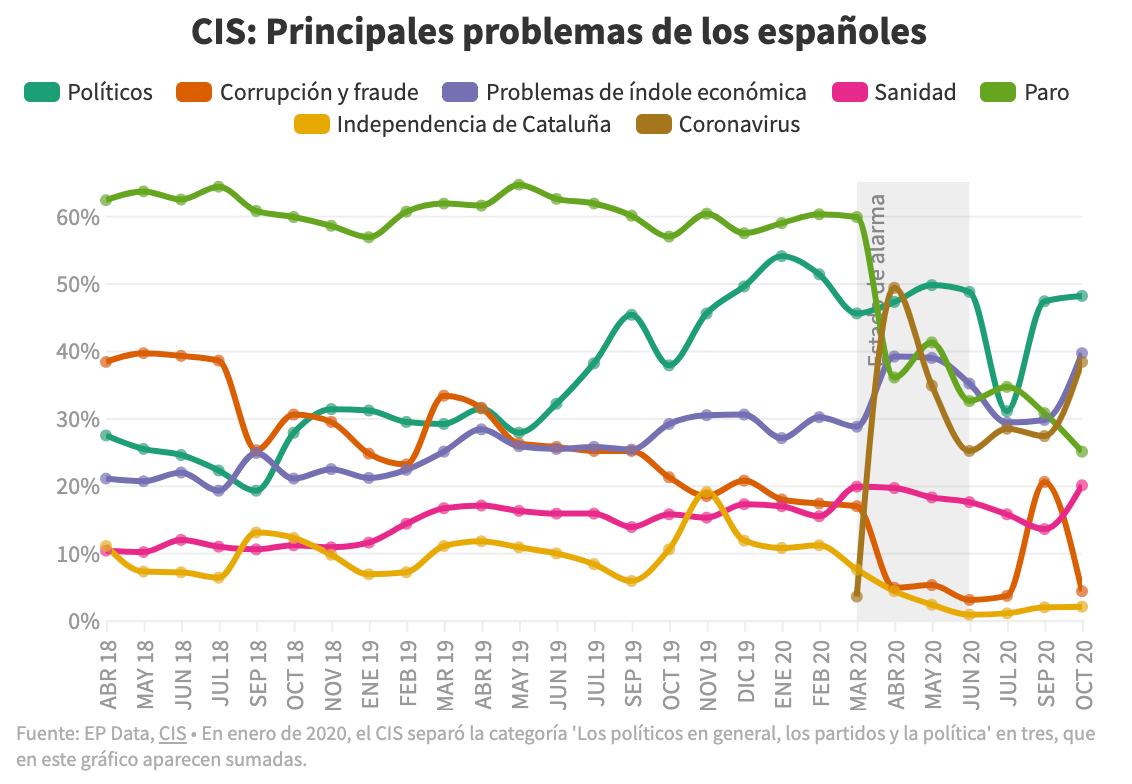
\includegraphics[scale=0.5]{doc/logos/imgs/CIS_1.png}
	\caption{ \cite{rtve-cis}  Principales problemas de los españoles según el CIS }
    \label{fig:worst_f_value}
\end{figure}

Como podemos observar en la gráfica superior a pesar no estar exenta de movimientos sinusoidales 
en la preocupación de los españoles en la sanidad siempre se muestra con una tendencia al alta 
solo superada por el paro y problemas de índole económico. 
Es evidente que la mejora del sistema sanitario es algo que nos concierne y repercute 
directamente en todos nosotros.

La ideación de un sistema que utilice datos publicados por el INE\footnote{Instituto Nacional de Estadística} sobre las defunciones según 
la causa de muerte para obtener un análisis inteligente que nos permita conocer, obtener y predecir
como han avanzado este tipo de decesos a lo largo del tiempo puede suponer una pequeña mejora de 
nuestro Sistema Nacional de Salud en materia de prevención y promoción de la salud. Es necesario que el 
SNS sea capaz de realizar cribados preventivos más inteligentes mediante el conocimiento fáctico autogenerado.

\section{Objetivos}
El principal objetivo de este Trabajo Fin de Grado consiste en obtener un sistema de análisis de datos que nos aporte
información enriquecida sobre los datos publicados por el Instituto Nacional de Estadística sobre las causas de muerte. 
Para conseguir el resultado final esperado debemos cumplir los siguientes objetivos:
\begin{itemize}
    \item Desarrollo de un modelo de datos que se adapte a los datos ofrecidos por el INE.
    \item Diseño y creción de una interfaz de programación de aplicaciones que ofrezca los datos procesados y 
filtrados a petición de usuarios o aplicaciones de terceros.
    \item Proveer de un punto de acceso visual para obtener gráficas y predicciones sobre los datos.
\end{itemize}

Una vez finalizado todo el proceso, además de haber obtenido la posibilidad de obtener la información 
desde un punto de acceso. Abrimos la posibilidad a usuarios experimentados de poder usar esta API para 
integrarla en sus soluciones o publicar los datos en los distintos formatos que nuestra API ofrece 
siempre que se mantenga la licencia original de publicación.



	% Estado del arte
	% 	1. Crítica al estado del arte
	% 	2. Propuesta
	\chapter{Estado del arte}

En este apartado lo que pretende es mostrar como se encuentra el panorama en el cual vamos a llevar a cabo este proyecto. Para ello, en primer lugar voy a analizar soluciones similares ya existentes, de forma que analicemos los requisitos de nuestro sistema comparándolo con aquellos que ya existen para obtener nuestra propuesta de valor.

\section{Análisis de mercado}

Como he comentado ya con anterioridad, el acceso a los datos sobre las defunciones es de dominio público, se puede encontrar información al respecto en los sitios que voy a exponer a continuación. Cualquiera puede acceder a ellos y verlos, el principal problema surge cuando queremos hacernos preguntas en base a esos números que vemos. Hasta que nivel se adaptan los sistemas existentes a las necesidades de mis usuarios. Vamos a ver las principales fuentes que existen y lo que nos ofrecen para a continuación, saber que tipo de tratamiento informático necesitamos realizar para satisfacer las necesidades de estos.

\subsection{Instituto Nacional de Estadística}
Uno de los primeros sitios en los que consulté fue la página del \href{https://www.ine.es/index.htm}{Instituto Nacional de Estadística} que es un referente en España en cuanto a la coordinación de servicios estadístico.
En este \href{https://www.ine.es/jaxiT3/Tabla.htm?t=6609}{enlace} se pueden observar las defunciones según causa de muerte filtradas por causa, sexo, edad y periodo. 
Enumero las principales desventajas encontradas desde el punto de vista de mis usuarios:
\begin{itemize}
    \item No permite realizar consultas a los datos.
    \item No soporta ningún protocolo para obtener agnósticamente estos datos y poder usarlo en otros softwares/aplicaciones.
    \item Poca precisión de filtrado por las pocas variables de las que disponemos.
    \item No tenemos visualización gráfica. Te redirige a descargar el programa PC-Axis únicamente disponible para Windows si quieres ver mas detalles sobre los datos almacenados.
\end{itemize}
\FloatBarrier
\begin{figure}[]
	\centering
	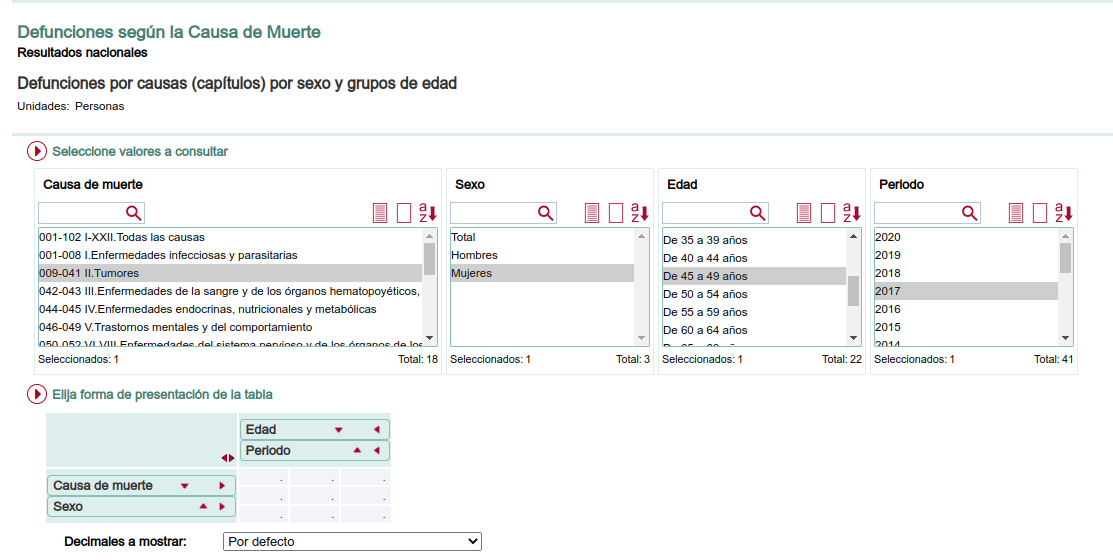
\includegraphics[scale=0.5]{doc/logos/imgs/ine1.png}
	\caption{  Vista principal para obtener datos en el INE }
    \label{fig:worst_f_value}
\end{figure}

\begin{figure}[]
	\centering
	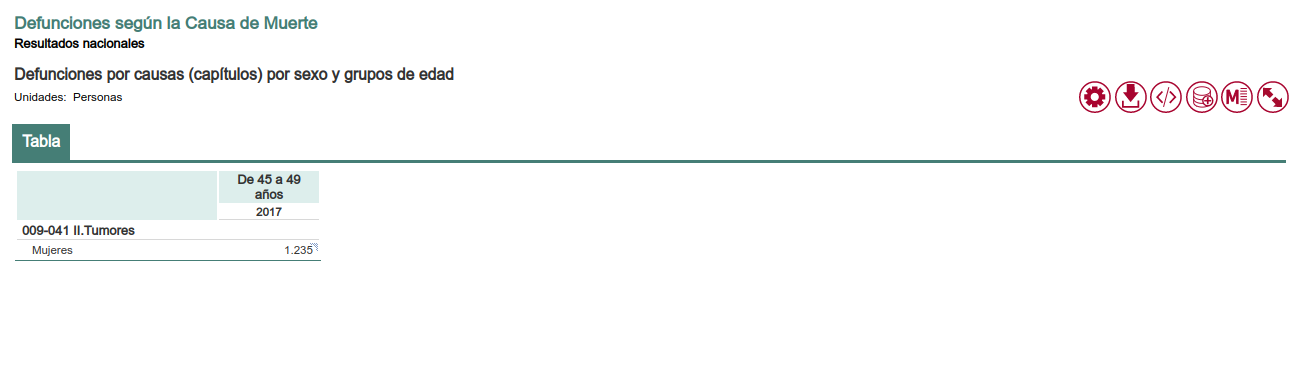
\includegraphics[scale=0.5]{doc/logos/imgs/ine2.png}
	\caption{ Vista resultado cuando se han filtrado los datos a obtener }
    \label{fig:worst_f_value}
\end{figure}
\FloatBarrier

\subsection{Instituto de Salud Carlos III}
En la página del Instituto de Salud Carlos III \footnote{https://www.isciii.es/Paginas/Inicio.aspx} podemos encontrar muchas entradas  hablando sobre \Gls{mortalidad} de la población y \Gls{morbilidad} apoyada de \Gls{momo} \href{https://www.isciii.es/QueHacemos/Servicios/VigilanciaSaludPublicaRENAVE/EnfermedadesTransmisibles/MoMo/Paginas/default.aspx}{Instituto de Salud Carlos III - Vigilancia de la Mortalidad Diaria} que son gráficas de desviaciones de mortalidad diaria respecto a la esperada según las series históricas de mortalidad, estas constituyen un sistema de vigilancia que proporciona información sobre el impacto en mortalidad de la población. Estas son entregables en formato web y PDF.

A pesar de la valiosísima información que estos informes pueden arrojar, sobre todo desde el punto de vista sanitario. Esto no es lo que persigue satisfacer en este trabajo, que se centra en facilitar la obtención de datos crudos. El instituto pone a disposición de los ciudadanos dos servidores.

\subsubsection{Servidor Arïadna}
Nos permite consultar información sobre las causas de defunción atendiendo a cuatro variables: Indicador, Causa, Período y años. Estas variables son las disponibles desde la interfaz web.
Y los indicadores pueden ser:
\begin{enumerate}
  \item Tasa ajustada a la población europea.
  \item Tasa ajustada a la población mundial.
  \item Tasa truncada: tasa ajustada de mortalidad limitada a los 35-64 años de edad.
  \item Índice comparativo de mortalidad: Es el cociente entre la tasa ajustada por edad en cada provincia y la tasa
  ajustada para el conjunto de España.
  \item Tasa cruda: la tasa cruda de mortalidad es la proporción de personas que fallecen con respecto al total
  de la población en un período determinado. Se expresa habitualmente como el número de defunciones al año
  por cada 100.000 personas.
  \item Número de defunciones
\end{enumerate}
\FloatBarrier
\begin{figure}[]
	\centering
	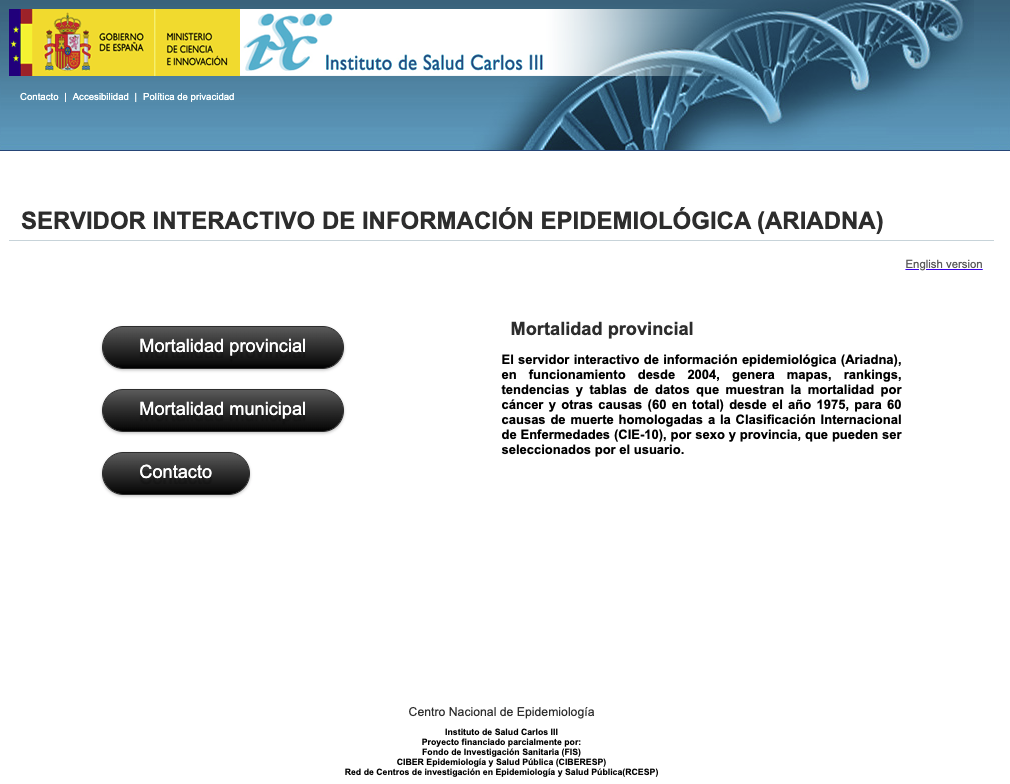
\includegraphics[scale=0.3]{doc/logos/imgs/ariadna1.png}
	\caption{ Vista principal del \href{http://ariadna.cne.isciii.es/}{servidor Arïadna} }
    \label{fig:worst_f_value}
\end{figure}

\begin{figure}[]
	\centering
	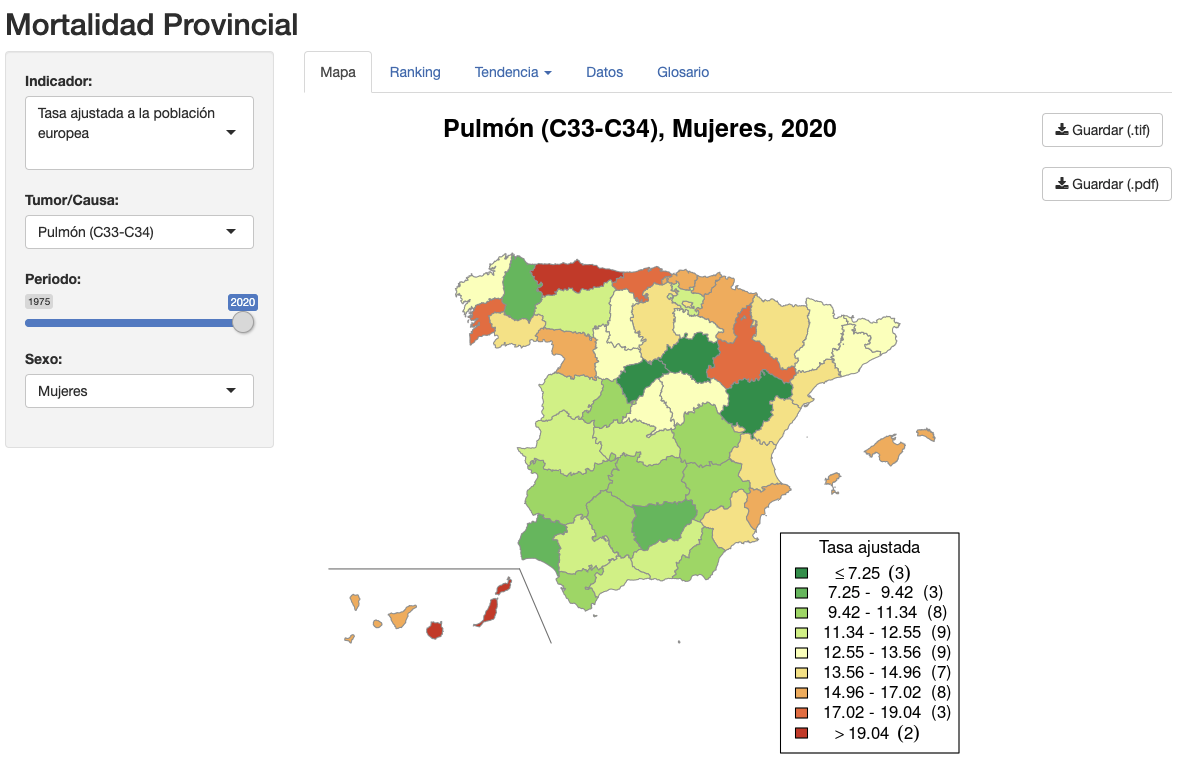
\includegraphics[scale=0.3]{doc/logos/imgs/ariadna2.png}
	\caption{ Vista por mortalidad provincial del servidor Arïadna }
    \label{fig:worst_f_value}
\end{figure}
\FloatBarrier
Los datos son ofrecidos mediante un mapa de España interactivo podemos observar también gráficas de todas las provincias y la media nacional así como una tabla con los datos. Es de obligado comentar la antigüedad manifiesta de la página y la poca agilidad con la que cargan los contenidos.
Esta página permite descargarse los datos únicamente en formato CSV y sólo de 10 tuplas en 10 tuplas sobre las  variables filtradas. Lo que sigue dificultando el acceso completo a cualquier interesado.

\subsubsection{Servidor Raziël}
Es un servidor interactivo \footnote{http://raziel.cne.isciii.es/index.php} que genera mapas y gráficas de España por comunidades autónomas, y tablas de datos que muestran las diferencias en la mortalidad por diversas causas. Ofrece datos desde el año 1980, de acuerdo con los criterios que de el usuario.
La web nos permite consultar las gráficas citadas anteriormente atendiendo a cuatro variables:
\begin{enumerate}
    \item Indicador.
    \item Causa.
    \item Período, años.
    \item Sexo.
    \item Grupo de edades.
    \item Comunidad Autónoma.
\end{enumerate}

Estas variables son las disponibles desde la interfaz web. Además, la web es prácticamente inaccesible e imposible de obtener los datos en tablas o en algún formato descargable por lo que no me quedó otra opción más que contactar con los servicios informáticos del instituto.


\section{Mi propuesta ante el estado del arte}

Sin perder de vista los \hyperref[sec:obj]{objetivos} y \hyperref[sec:usu]{usuarios diana} a utilizar este trabajo.  ha sido una tarea útil y fundamental contrastar las "soluciones" existentes para darme cuenta de que los datos no son nada accesibles ni para científicos para que puedan desarrollar estudios ni prácticamente para usuarios observadores ya que la antigüedad de los sistemas, el tiempo de carga y lo nula inversión en accesibilidad hace imposible su uso.

Tras ponerme en contacto con los servicios informáticos del instituto, no tuvieron problema alguno en pasarme todos los ficheros de los que se sirve el servidor, de hecho me llevé una grata sorpresa al ver que almacenaban más variables de las que ellos ofrecían, lo que me ha permitido hacer un trabajo más rico. En el capítulo 5: Análisis de los datos, lo analizaremos más en detalle.


Para terminar con mi propuesta, he recogido someramente los siguientes puntos en los que ha de guiarse la solución. Las principales deficiencias encontradas y objetivo a subsanar son:
\begin{itemize}
    \item Inexistencia de una interfaz de consulta para que usuarios externos puedan obtener los datos de forma uniforme y utilizando protocolos actuales.
    \item Los datos expuestos en la web no son completos, por razón que desconozco no se muestran todas las variables existentes.
    \item No permite realizar consultas conjuntas a los datos.
    \item La visualización gráfica no se consigue por todas las variables.
\end{itemize}

	
	\chapter{Planificación}
En este capítulo detallaré todo lo relativo a la planificación y estimación del proyecto. 

\section{Metodología utilizada}
Desde que se empiezan a programar los primeros ordenadores en la historia, la programación siempre ha sido 
minguneada y considerada bastante lejos de una actividad científica. Todo empezó a cambiar cuando los scripts
permitían realizar cálculos como ninguna otra herramienta hasta el momento. Fue la matemática Margaret Hamilton 
quien planteó por primera vez que los sistemas informáticos tenían que integrar tres componentes: hardware, 
software y los usuarios que los iban a usar. Fue Margaret Hamiltonen, cuando se produce lo que conocemos como 
crisis del software en 1968 quien acuñó en la \textit{NATO Software Engineering Conference} el termino Ingeniería
al proceso de creación de software. En ese momento donde parecía que crear software duradero y escalable en el tiempo 
era misión imposible hizo que se invirtiera en investigación y se construyera conocimiento. Este conocimiento es lo que hoy 
llamamos Ingeniería de Software: herramientas, técnicas de especificación y diseño que nos permiten especificar, 
desarrollar, validar y evolucionar como en cualquier otra ingeniería.

Las metodologías ágiles presentan una forma distinta de trabajar y organizarse, adaptándose a las condiciones
cambiantes que puedan surgir, aprovechando estos cambios para obtener ventajas. Con este tipo de metodologías 
podemos dividir el trabajo en pequeñas piezas de manera que podemos ir realizándolos de forma incremental.

Se ha barajado utilizar una de las dos metodologías más empleadas en la industria: Scrum y eXtreme Programming. 
eXtreme programming ha sido descartada por la imposibilidad de aplicación en términos de tiempo y recursos humanos. 
Los roles y artefactos exigidos por esta metodología son indiscutiblemente para un equipo de desarrollo segmentado. 
Sin embargo y en comparación con Scrum es una metodología muy enfocada en el proceso de desarrollo. Obliga a 
desarrollar guiándose de pruebas, a programar en parejas y asegurar la calidad del código en todas las etapas.

Scrum en cambio se muestra más flexible. En el año 2001 que K. Schwaber y Mike Beedle publican el
primer libro sobre Scrum\cite{agile_book}: "Agile Software Development with Scrum" esta metodología se ha convertido en la
más utilizada para el desarrollo de software. Siendo precisos y prudentes tampoco es posible aplicar 
propiamente dicho Scrum en este proyecto... fundamentalmente por ser una persona a cargo de todo el proceso.

Por tanto, me he permitido crear mi propia metodología de desarrollo basándome en los tres valores fundamentales 
que ofrecen estas tecnologías:
\begin{itemize}
    \item \textbf{Transparencia}: en todo momento se ha de conocer en qué se está trabajando, que problemas se está teniendo y/o si 
    existe algún bloqueo asociado.
    \item \textbf{Inspección}: se ha de inspeccionar y no perder de vista el progreso para conseguir el objetivo. La 
    trazabilidad del trabajo nos la ofrece el SCV (source control versioning) en nuestro caso GitHub con incorporación
    de funcionalidad por pull request.
    \item \textbf{Adaptación}: poder reaccionar a tiempo a los cambios requeridos por los stakeholders.
\end{itemize}

Una buena forma de cumplir las características citadas anteriormente, es realizar el desarrollo guiado por pruebas, 
lo que se conoce por TDD, \textit{Test Driven Development}. Al emplear esta metodología garantizamos la calidad 
de lo programado, trasladamos los requisitos a las pruebas de forma que se convierten en la más fiable documentación.
Además tener una gran cobertura de código testeado nos permite poder refactorizar con asiduedad y garantizarnos 
no generar mucha deuda técnica.
Como se ha comentado en otro capítulo de esta memoria, este trabajo quiere prestarle especial atención al 
automatizaje de tareas y trabajos de infraestructura, la realización de un sistema que se integre continuamente 
(CI) hace que se proteja siempre el PMV ya que es requisito indispensable para seguir añadiendo funcionalidad 
que los test pasen lo que significa que se siguen manteniendo los requisitos anteriores al añadir nueva 
funcionalidad.

\section{Herramientas}
Para el contribuir con la segunda característica introspectiva citada anteriormente, necesitamos no perder
de vista el progreso para conseguir el objetivo. Se ha recurrido a utilizar un sistema de control de versiones,
sin discusión alguna GIT ha sido la herramienta seleccionada. Se hace necesario una forja donde respaldar nuestro 
código, GitHub ha sido la opción seleccionada para alojar el código y tener un registro de las issues y Pull Request. Estas
características también las pueden servicios como GitLab. Pero las características premium de GitHub que ofrece una cuenta
universitaria como los tableros Kanban, integración continua con GitHub Actions...

Haciendo uso de esta herramienta, se han definido unas serie de milestones que agrupan historias de usuario e issues o tareas a realizar. Los
incrementos en el trabajo se han ido realizando por medio de Pull Request y cada una de estas lleva enlazada una o varias
issues. Para tener una visión general del estado del proyecto se ha usado la herramienta Projects integrada en GitHub.

\subsection{Milestones}
Los milestones hacen referencia al conjunto de productos mínimamente viables que se van generando conforme se avanza en el
desarrollo del proyecto. Un milestone está formado por un conjunto de issues, se entiende finalizado un milestone cuando se
han contemplado todos los issues asociados.
Los milestones creados se pueden observar en el repositorio de GitHub y son los siguientes:
\begin{enumerate}
    \item \textbf{Infraestructura}: desarrollo de la integración continua que compila la memoria y comprobador ortográfico más
    historias de usuario iniciales.
    \item \textbf{Modelo de datos}: definición de las clases que conforman el dominio del problema, atendiendo al estado
    del arte. El PMV incluye también las redacciones pertinentes de los capítulos de la memoria y el pretexto a las decisiones
    técnicas elegidas para implementar la solución.
    \item \textbf{Interfaz de programación de aplicaciones}: es la estructura del modelo que representa la solución del problema
    y todas las operaciones posibles a realizar con ellas. Supondrá la capa de abstracción para acceder a los datos y que pueda
    ser utilizada por otros desarrolladores para construir aplicaciones con distintos objetivos.
    \item \textbf{Frontend}: creación de un sistema web que permita consumir el API satisfaciendo las necesidades de mis usuarios ficticios.
\end{enumerate}

\subsection{Historias de usuario}
Como estamos trabajando con una metodología de desarrollo ágil queremos expresar las necesidades reales del sistema para
lograr la interacción del equipo de desarrollo con el usuario. Todas las historias de usuarios están definidas en un milestone
de trabajo y de ellas se generarán tareas específicas. La especificación de las historias de usuario e issues generadas a partir de ellas
pueden verse con mayor detalle en el panel de \textbf{Issues} del repositorio de GitHub.
\begin{figure}[]
	\centering
	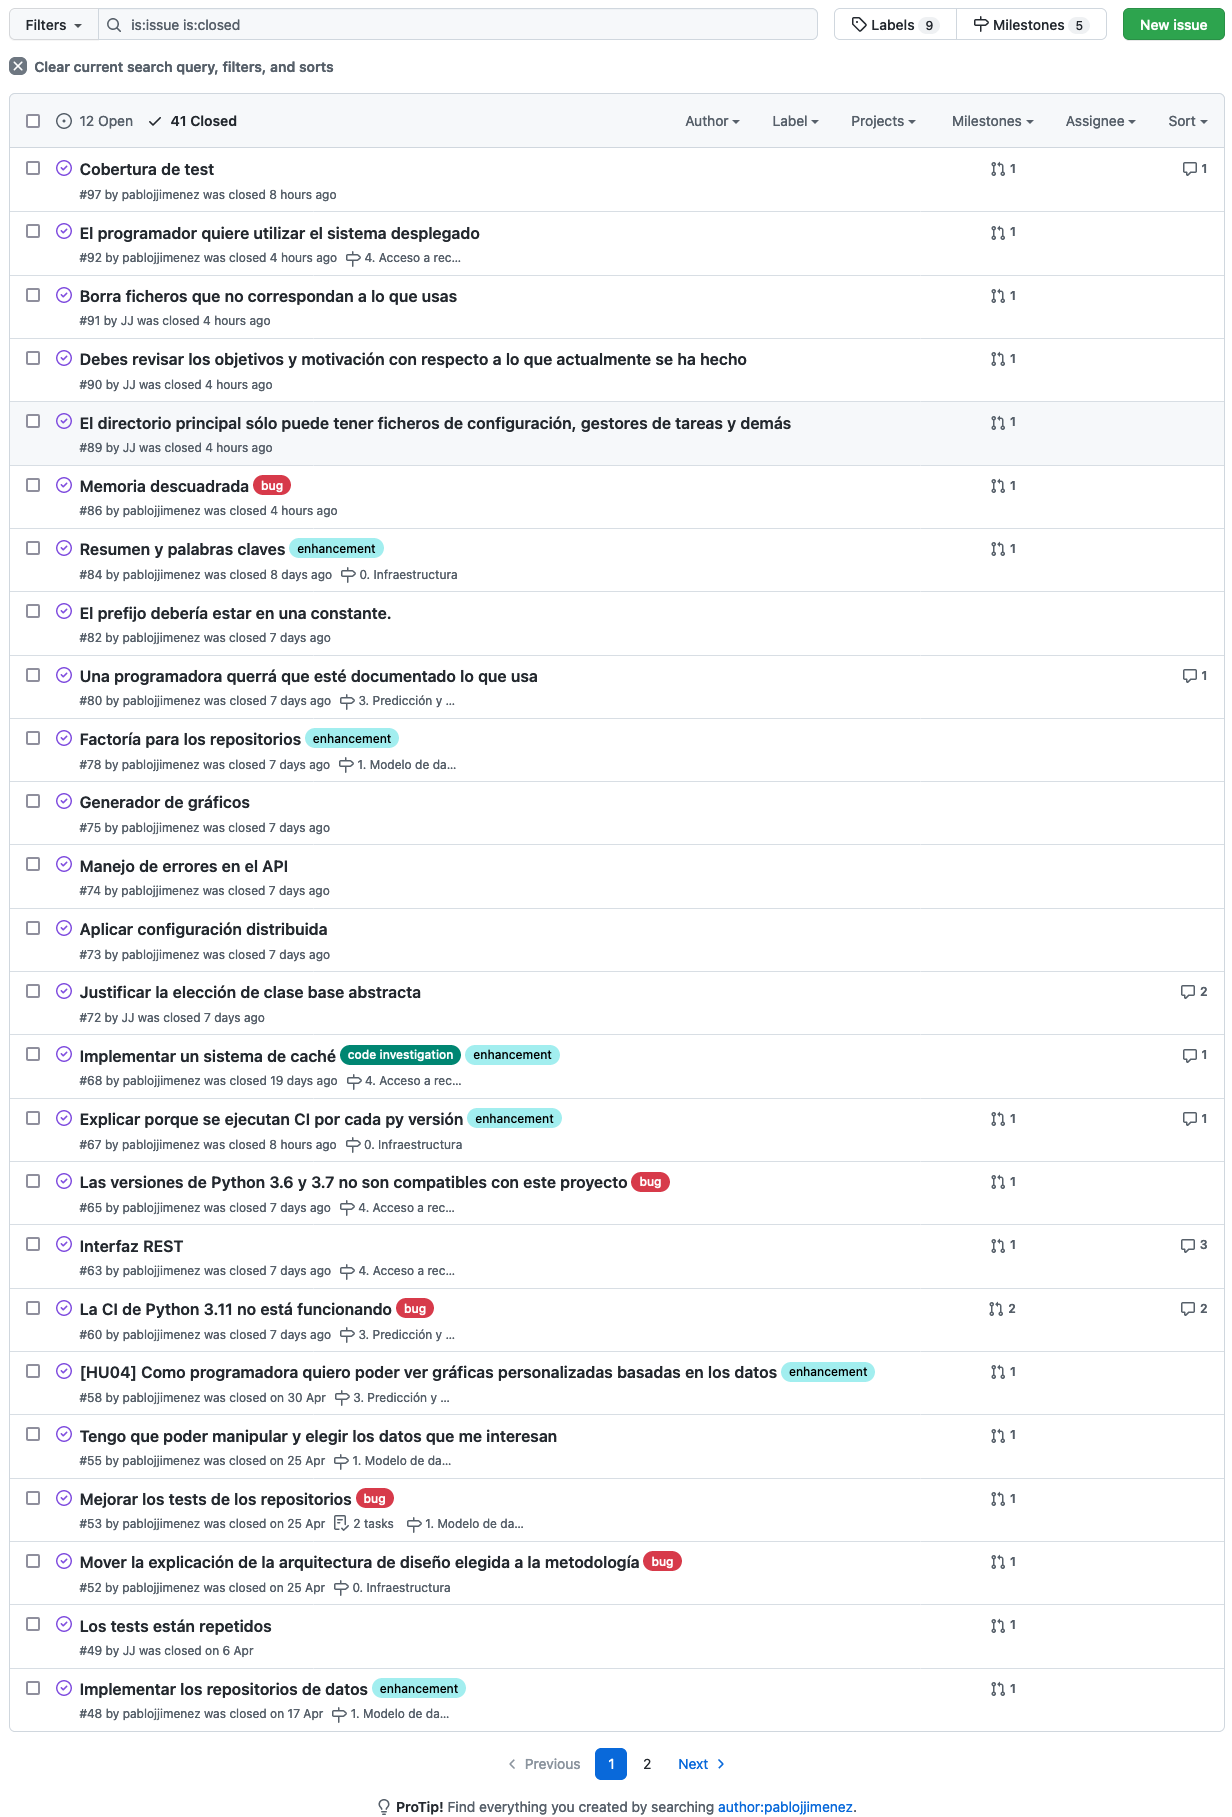
\includegraphics[scale=0.5]{doc/logos/imgs/issues.png}
	\caption{ \cite{rtve-cis}  Issues del TFG vistas desde el correspondiente \href{https://github.com/pablojjimenez/TFG/issues}{panel en GitHub}. }
    \label{fig:worst_f_value}
\end{figure}

\section{Temporización}
[TODO: Añadir diagrama de Gantt]

\subsection{Cuantización de las horas empleadas}
[TODO: añadir algún gráfico procedente del CSV que vamos realizando]

\section{Estimación de costes}
A partir de la información anterior en cuanto al tiempo invertido en el proyecto y en vista de los elementos necesarios
para llevarlo a cabo podemos detallar los costes asociados que tendría la elaboración del proyecto.

\begin{itemize}
    \item Nómina para el ingeniero junior.
    \item MacBook Pro [amortizado 5 años]: 240€
    \item Recursos software utilizados han sido gratuitos.
    \item Recursos de despliegues han sido gratuitos.
\end{itemize}

	% Análisis del problema
	% 1. Análisis de requisitos
	% 2. Análisis de las soluciones
	% 3. Solucion propuesta
	% 4. Análisis de seguridad
	\chapter{Análisis de los datos disponibles}
\label{cap:5}
Los datos acerca de las defunciones son un componente fundamental en este trabajo sin el
cual no podríamos construir nuestra solución. Si bien es cierto que no es difícil obtener
estos datos del Instituto Nacional de Estadística, estos son demasiados pobres, no nos
ofrecen bastante información para poder construir una solución con suficiente
semántica.

Durante la documentación del \hyperref[sec:estadoArte]{capítulo anterior}, descubrí que el
Instituto Carlos III recolectaba e intentaba exponer estos datos con mucho más detalles
que los anteriores. Tras conocer la existencia de los servidores Arïadna y Raziël me puse
en contacto con el \textbf{Instituto de Salud Carlos III} por correo electrónico para que
me compartieran estos datos de dominio público\footnote{Son los datos almacenados en el
servidor interactivo Arïadna y Raziël comentados en el capítulo sobre el estado del arte.
\hyperref[sec:estadoArte]{Enlace al capítulo}} almacenados en sus servidores. Esta
colección de datos sí es muy completa, nos ofrece muchos tipos de enfermedades y nos ofrece
información normalizada.

Estas son las columnas normalizadas:
\begin{enumerate}
\item \textbf{AVP}: Años potenciales de vida perdidos.
\item \textbf{CRUDA}: Tasa bruta.
\item \textbf{TAVP}: Tasa de años potenciales de vida perdidos.
\item \textbf{EDAD}: Edad media de la defunción.
\item \textbf{TASAE}: Tasa ajustada a la población europea.
\item \textbf{TAVPE}: Tasa ajustada de años potenciales de vida perdidos.
\item \textbf{TASAW}: Tasa ajustada a la población mundial.
\item \textbf{TASAVPW}: Tasa ajustada de años potenciales de vida perdidos.
\end{enumerate}

El resto de columnas que forman los datos son:
\begin{enumerate}
\item \textbf{ANO}: Año de consulta (1980 a 2020).
\item \textbf{CAUSA}: Código de la causa.
\item \textbf{SX}: Sexo (1: hombres, 2: mujeres).
\item \textbf{CCAA}: Comunidad Autónoma.
\item \textbf{GEDAD}: Grupos de edad.
\item \textbf{DEFU}: Número de defunciones.
\end{enumerate}

La representación de estos datos la he denominado \textbf{Decease} integra otros modelos como
la causa (motivo de la defunción) que es un objeto formado por el nombre de la causa y su
equivalencia con el estándar \gls{CIE-10} que es el acrónimo de la Clasificación
Internacional de enfermedades en su 10.ª edición.

La principal diferencia aparente que existe entre la información que sirve
\textbf{Arïadna} y la de \textbf{Raziël} es que Arïadna no guarda información acerca de los
grupos de edades, solo nos ofrece el cómputo de la edad media. Este cómputo podemos
calcularlo nosotros conociendo los rangos de edad. Por tanto descarté Arïadna sospechando
que es la misma fuente que Raziël pero con algunas columnas calculadas.

	% Desarrollo bajo sprints: 
	% 	1. Permitir registros y login de usuarios
	% 	2. Desarrollo del sistema de incidencias
	% 	3. Desarrollo del sistema de denuncias administrativas y accidentes
	% 	4. Desarrollo del sistema de croquis
	%   5. Instalación de la aplicación de manera automática
	\chapter{Desarrollo de la solución}
A la hora de empezar con la implementación de la solución, debemos comenzar teniendo en cuenta la arquitectura software que satisface requisitos del sistema de acuerdo con los usuarios. Es decir, con las historias de usuario que han expresado.

\section{Arquitectura software de la solución}
Para el diseño del software se ha utilizado el diseño dirigido por el dominio, DDD \textit{Domain Driven Design}. Este tipo de arquitectura introducida por Eric Evans \cite{ddd_book} "Domain-Driven-Design - Tackling Complexity in the Hearth of Software, 2004" nos permite organizar el código de forma separada y organizada lo que nos permite poder realizar TDD correctamente ya que por tener las distintas capas separadas y débilmente acopladas unas de las otras. Gracias a este bien diseño es muy fácil hacer uso de la inversión de dependencias \footnote{https://jj.github.io/curso-tdd/temas/inversi\%C3\%B3n.html} para inyectar en los tests las clases \textit{mockeadas} \footnote{El término mockear en desarrollo de software se refiere a reemplazar o imitar a un objeto real. El propósito es que al probar el programa o hacer testing, podamos utilizar este mock para conocer su estado.} que necesitemos. 

La arquitectura dirigida por el dominio nos permite fácilmente aislar la lógica de negocio en un único sitio y siempre lo más cerca del dominio posible lo que nos permite cumplir los principios SOLID fácilmente y conseguir un código abierto a su extensión pero cerrado a su modificación.  

Un requisito fundamental expresado por los usuarios diana a utilizar este proyecto es poder desplegar fácilmente este proyecto en la nube, gracias a que se ha desarrollado utilizando capas desacopladas entre si, podemos distribuir en distintos clústeres \footnote{Nos referimos a la técnica por la cual podemos combinar un sistema para que trabaje paralelamente en un entorno cloud. Lo que conseguimos con esta operación es una mayor disponibilidad, más velocidad de despacho y escalabilidad del sistema. Como todo, a cambio tendremos un sistema más costoso de mantener económicamente y un mayor tiempo de implementación. } la implementación sin realizar prácticamente cambios en la implementación.  Es fundamental desacoplar al máximo todos los componentes y que cada uno tengo una única responsabilidad cuando se realiza un proyecto en la nube. La principal desventaja que podemos encontrar en este tipo de arquitecturas es la comunicación entre los distintos componentes.  Una solución a este problema podría ser la comunicación por eventos, potente pero compleja a nivel técnico y costosa económicamente. Otra solución es mediante inyección de dependencias, que es la que he empleado en este proyecto, podemos decir que la debilidad de esta solución reside en que una de las capas puede crecer en sobremedida y convertirse en un cuello de botella.



\subsection{DDD}
En este tipo de arquitectura donde diseñamos guiándonos por el dominio, podemos diferenciar tres elementos importantes.

\subsubsection{Entidad}
Las entidades son aquellas clases que representan una entidad del dominio. Estas clases deben tener una estructura de datos que represente la información de la entidad y unas responsabilidades concretas. Se caracterizan porque tienen que ser consideradas iguales a otros objetos aún cuando cuando sus atributos difieren. En las entidades se encuentran las restricciones del dominio, en ellas se realizan las validaciones de valor e integridad. Cualquier error o situación inválida hay que notificársela al sistema mediante una excepción. 

Definir y diseñar los estados inválidos de las entidades y de la aplicación en general es un apartado fundamental que debemos de realizar con el mismo cuidado que con el que diseñamos las entidades.

Este proyecto consta de dos entidades: \codeword{Disease} que representa a una enfermedad y \codeword{Raziel} que es sin lugar a duda el modelo más rico en información. Estas entidades poseen las restricciones de valor como puede ser el tipado de sus atributos o la satisfacibilidad solo de los valores que tienen sentido semántico. También restricciones de integridad como por ejemplo, que un objeto de tipo \codeword{Disease} puede tener el campo \codeword{cie}, nulo.

\subsubsection{Value objects}
Representan los conceptos que no tienen una entidad. Describen características por lo que solo nos interesan sus atributos.
Los value object representan elementos del modelo que se describen por el \textbf{qué} son, y no por \textbf{quién} o \textbf{cuál} son. Estos elementos completan y/o forman parte de las entidades del sistema.

En este proyecto la representación en código de las comunidades autónomas corresponde con un tipo de value object utilizado por la entidad \codeword{Raziel}

\subsubsection{Servicios}
No tienen significado propio suponen la capa que representa las operaciones que no pertenecen conceptualmente a ningún objeto del dominio concreto. 

En este proyecto, los servicios son el punto de entrada de las peticiones que le hace el usuario al sistema. Son también los encargados de arrancar todo el proceso de obtención de los datos.

\subsubsection{Repositorios}
Representan al conjunto de modelos y entidades. Se utilizan para almacenar u ofrecer los conjuntos de objetos. Suelen suponer una capa de abstracción sobre el sistema de almacenaje, ya sea una base de datos, unos ficheros en disco o incluso la invocación de otros servicios externos como puede ser un API. Esta parte es fundamental para poder modular y preparar las aplicaciones para cambiar de infraestructura sin tener que modificar el código de programación.

En este proyecto hemos implementado este concepto haciendo uso de un \codeword{AbstractRepository} representado por una clase abstracta. Debido a que, semánticamente no tiene sentido poder utilizar este tipo de repositorio en sí mismo. Sin embargo, es usado de clase padre para el resto de repositorios porque impone a las clases que lo heredan una interfaz uniforme de métodos y abstrae lógicas comunes a este tipo de concepto.

El proyecto está compuesto por cinco repositorios que obtiene en forma sus modelos correspondientes. Al existir este tipo de jerarquía y compartir todos estos el mismo tipo de operación, resulta idónea la aplicación del patrón de diseño de creación \textit{Factory Method}. Si bien es cierto, que es en lenguajes tipados donde este tipo de soluciones suponen un cambio radical en cuanto a la comodidad y encaje en la creación de instancias a lo largo del programa. A nosotros también nos mejora la calidad del código, pudiendo hacer uso de cualquier repositorio con una sola importación, ya que en otro caso habría que construir el repositorio \textit{in situ} e inyectarle todas las dependencias que necesitara.


\subsection{Diagrama arquitectónico de la solución}
A continuación se puede ver un somero diagrama donde podemos observar la conexión entre los distintos componentes del sistema y la conexión con librerías y frameworks externos. 

\begin{figure}[]
	\centering	
	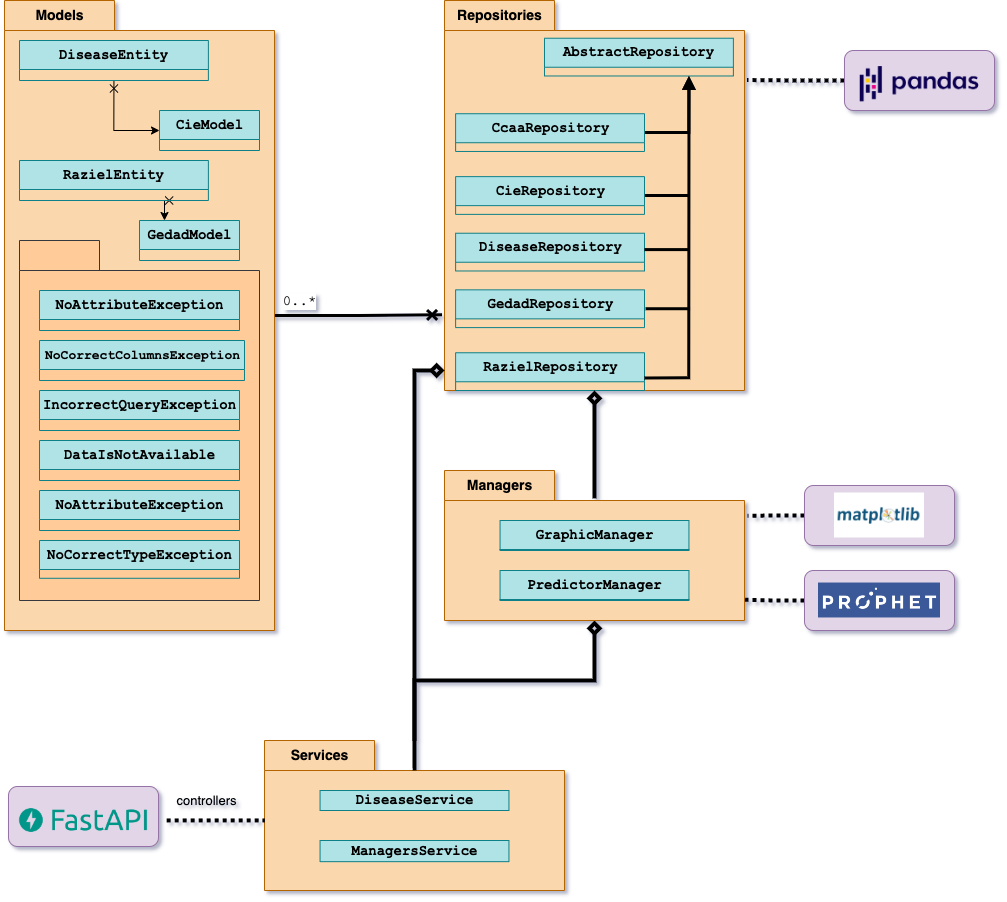
\includegraphics[scale=0.5]{doc/logos/imgs/arquitectonico.png}
	\caption{ \cite{rtve-cis} Modelo organizativo del código con sus dependencias externas. }
    \label{fig:worst_f_value}
\end{figure}



\section{Implementación}
\subsection{Lenguaje de programación}
El lenguaje elegido ha sido \textbf{Python} los motivos de esta decisión son variados, por los que procedo a enumerarlos:
\begin{itemize}
    \item Es un lenguaje que se encuentra en las \cite{tiobe} primeras posiciones como lenguaje más utilizado a día de hoy. Además me encuentro muy cómodo programando en él.
    \item Es un lenguaje que cuenta con muchísimas bibliotecas, muchas de estas especiales para trabajar con datos y ficheros (como \textbf{Pandas}). Abundan también los \textit{frameworks} que nos ayudan a construir APIs con él y la mayoría de PaaS \footnote{Platform as a Service} soportan este lenguaje.
    \item Es un lenguaje interpretado, débilmente tipado y con una capacidad introspectiva muy alta que nos permite metaprogramar.
\end{itemize}

A la hora de realizar un proyecto software siempre es necesario utilizar bibliotecas y código implementado por otras personas para poder llegar más lejos. Todo esto es lo que llamamos dependencias. Muchos entornos de programación tienen gestores de dependencias que nos permiten instalar y gestionar estas dependencias cómodamente. En el entorno JavaScript tenemos \textit{npm} o \textit{yarn} que nos permite instalar dependencias de forma sencilla. Para la JVM el tradicional \textit{maven} es una buena opción o la mas moderna y potente \textit{Gradle}.

En Python se ha extendido el uso de \textbf{Poetry} que de forma muy parecida a \textit{npm} genera un fichero de configuración \textit{pyproject.toml} donde definimos las dependencias, las versiones y los paquetes de nuestro proyecto así como algunas tareas específicas para correr los tests o el lint fácilmente. Esto facilita enormemente la creación de entornos virtuales de prueba y de desarrollo tanto el local como por el CI.

\subsection{Bibliotecas utilizadas}

\section{Para Continuos Integration}
Desde el inicio del trabajo se ha estado trabajando con un sistema férreo de CI de forma que no se ha mezclado nunca nada que no haya superado los requisitos de diseño especificados. En el entorno de desarrollo se ha utilizado \textit{Github Actions} que es una herramienta de CI que nos permite realizar una integración continua de la misma forma que \textit{Travis CI} la elección de Github sobre Travis es por la rapidez del elegido e integración con la forja utilizada que como se ha especificado anteriormente es Github.

Para garantizar la \textbf{calidad de la memoria} se han implementado dos tipos de CI\footnote{Continuos Integration}: un revisor ortográfico y un revisor de estructura que compila el documento automáticamente y pública el PDF generado en las \href{https://github.com/pablojjimenez/TFG/releases}{\textit{releases} del repositorio.}

Del mismo modo, para el \textbf{código} se han implementado otras dos CI que garantizan que cuando se introduce en la rama principal del repositorio código nuevo, éste garantiza unos estándares de calidad y que efectivamente el código es funcional por todas las versiones especificadas de Python. Por un lado, verificar el código fuente contra errores de programación (como "library imported but unused" y "Undefined name") y para verificar la complejidad ciclomática. Se ha utilizado la tecnología \cite{flake}\textbf{Flake8} por ser las más utilizada en el ecosistema.
Por otro lado, se corre la \textit{suit} de tests de forma que se garantice que al añadir uno código no se rompe el existente. Se ha utilizado la librería \textit{Unittest} que se encuentra incluida en la biblioteca estándar de Python permite realizar aserciones, provee de muchas aserciones y permite organizar los tests de forma parecida a como lo hace jUnit en clases que llamamos \textit{suits} de tests.

Todas estas comprobaciones se realizan para todas las versiones de Python en las que garantizamos que el software funciona.

\subsubsection{Pandas}
Como se ha descrito en anteriores capítulos de la memoria, los datos que manejamos están en ficheros CSV. Para poder trabajar con ellos es necesario utilizar una biblioteca que nos permite trabajar con estos ficheros. Es necesario poder manejar los datos de estos ficheros con cierta agilidad. El mayor fichero tiene 967360 líneas y ocupa unos 55 MB aunque no son cifras cercanas a lo que se considera \textit{big data} necesitamos de una herramienta que nos permita filtrar, ordenar y hacer cálculos eficientemente sobre estos conjuntos de datos. La elección de \textbf{Pandas} como biblioteca para trabajar con estos datos es debido a que es ampliamente utilizada en el mundo Python y encaja en los datos que tenemos.

\subsubsection{Matplotlib}
Es una biblioteca para crear todo tipo de gráficos, es muy utilizada en el ecosistema Python y además ha sido elegida por su compatibilidad con \textit{Pandas} que permite realizar gráficas a partir de objetos Dataframe propios de la biblioteca \textit{Pandas}

\subsubsection{Prophet}
Es necesario poder obtener predicciones basadas en series temporales. Busco que la predicción sea rápida. Sea automática de forma que no haya que configurar muchos parámetros y que el pronóstico que ofrece sea ajustable; esto es, que permita modificar y ajustar los pronósticos agregando conocimiento del dominio.

La primera opción y más famosa en el lenguaje Python es scikit-learn, una biblioteca open source de machine learning que ofrece infinidad de algoritmos: de clasificación, regresión, clustering, selección de modelos, preprocesado...

Por otro lado, tenemos Prophet una biblioteca open source para Python y R desarrollada por Meta. Sus posibilidades son mas limitadas que las que nos ofrece scikit-learn pero por el contrario es muy básica y sencilla tanto de instalar como de usar. Además, su funcionalidad es justo la que buscamos, poder realizar predicciones sobre series temporales.

En Prophet, los modelos se ajustan usando Stan, otra biblioteca de inferencia estadística bayesiana con estimación de verosimilitud penalizada.

\subsubsection{FastAPI}
En aras de que el usuario pueda utilizar estos servicios de forma agnóstica sin tener que descargarse el código fuente e incluirlo en su proyecto a modo de biblioteca. Algo que por otra parte, supondría una gran restricción ya que el lenguaje de programación tendría que ser Python.

Para ello, se ha implementado una interfaz de comunicación REST. Como bien es sabido, los servicios restful se apoyan del estándar HTTP y por tanto, hereda sus conocidas características. REST es \textit{stateless} cada vez que utilizamos un recurso necesitamos ofrecerle toda la información identificativa pues carece de memoria, utiliza el formato JSON para el intercambio de datos y expone una serie de recursos o \textit{endpoints} que son las operaciones disponibles a realizar.

En el universo Python existen dos grandes frameworks para construir servicios restful: Flask y FastAPI.
Flask es un microframework, que dispone de multitud de complementos lo que te permite construir cualquier servicio configurando correctamente todos estos complementos. 

FastAPI es un proyecto de código libre mas moderno, de alto rendimiento, según la documentación \footnote{https://fastapi.tiangolo.com} oficial se podría igual al rendimiento que ofrece NodeJS o Go. Además, nos permite por defecto programar de forma asíncrona (muy interesante cuando hay acceso a bases de datos) y nos proporciona de forma automática una documentación OpenAPI.

La API de este software expone dos blueprints \footnote{Llamamos blueprint al conjunto de recursos que comparte el mismo prefijo de URI (Identificador de recursos uniforme)}

\begin{itemize}
    \item \textit{/data} Definido por el conjunto de recursos disponibles. Todos ellos aceptan los siguientes parámetros en la cabecera de las peticiones \codeword{sort} para ordenar los datos en base a algún campo, \codeword{limit} para limitar la cantidad de datos (por defecto se entregan limitados a 100 elementos), \codeword{page} para especificar la página.
    Y la siguiente estructura JSON como cuerpo de la petición:
    \begin{verbatim}
        {
            "ID": {
                ">": 1,
                "<": 3
            },
            "CIE": {
                "==": ""
            }
        }
    \end{verbatim}
    En este caso estaríamos indicando que queremos los elementos cuyos IDs se encuentran en el rango ]1, 3[ y cuyo campo CIE es vacío. Los operadores válido son: \codeword{==}, \codeword{<}, \codeword{>}

    \item \textit{/managers} Dispone de tres recursos. Uno para generar gráficos lineales (ver figura): requiere dos variables como parámetros en la cabecera, una para indicar la agrupación y otra para la suma, como cuerpo de la llamada podemos pasar una query con la estructura especificada anteriormente. Por último, tenemos dos recursos para obtener la predicción y la gráfica ajustada en el tiempo que indiquemos.
\end{itemize}

\subsubsection{Documentación de la API}
Con la ayuda de los recursos que pone a nuestra disposición FastAPI, se ha implementado una especificación OpenAPI. Esta especificación define una serie de propiedades en un formato legible por una máquina (suele usarse el formato JSON o YAML).

Gracias a eso podemos generar una documentación basada en HTML que nos permite conocer los recursos epuestos de la API, los argumentos y las estructuras de las respuestas esperadas. 

	% Presupuesto

	% Conclusiones
	\chapter{Conclusiones y trabajos futuros}
Al principio de este documento se definieron unos objetivos a alcanzar, vamos a analizar
en este capítulo si se han cumplido y cuales serian las lineas de trabajo futuras de
acuerdo con las necesidades expresadas por nuestros usuarios.

El principal reto que tenía que satisfacer este trabajo era la exposición de estos datos
de dominio público para que los usuarios diana fueran capaces de poder conocer la
evolución de las causas de muerte. Esto se ha conseguido implementando una serie de
interfaces agnósticas que permiten acceder al sistema desplegado y realizar consultas sin
necesidad de ningún tipo de configuración. 

Esto avanza en la necesidad de mejora que tiene el SNS para prevenir el máximo número
posible de muertes gracias a las aplicaciones integrales que pueden ser desarrolladas
utilizando este sistema.

Me siento orgulloso de haber sido capaz de realizar con éxito un proyecto de ingeniería de
software desde sus inicios, objetivos, planificación de recursos hasta estructurar una
metodología basada en desarrollo ágil que me ha permitido aportar valor inmediato en las
iteraciones y todo lo que he aprendido que pasa desapercibido en otras situaciones.

\section{Trabajos futuros}
Voy a exponer la principal línea de trabajo por la que sería -bajo mi opinión- interesante seguir:
\begin{itemize}
    \item Permitir la integración de distintas fuentes de datos con otros modelos de datos
    también distintos. Por ejemplo, con otras escalas temporales.
\end{itemize}
Este proyecto es libre y está publicado con licencia \cite{gplv3} por lo que, en
correlación también con el desarrollo ágil, cualquier usuario puede abrir tareas y
proponer cambios.

	% Trabajos futuros


	
	\newpage
	\bibliography{bibliografía}
	\bibliographystyle{plain}
	
\end{document}

